\documentclass[a4paper,openright,12pt,oneside]{article}
\usepackage[left=3cm,top=3cm,right=2.5cm,foot=3cm]{geometry} %marcos

%Paquetes
\usepackage{setspace}
\usepackage[nottoc]{tocbibind}
\usepackage[utf8]{inputenc}
\usepackage{graphicx}
\usepackage{subfig}
\usepackage{ragged2e}
\usepackage{amssymb,amsmath}
\usepackage[scr]{rsfso}
\usepackage{float}
\usepackage[spanish,es-tabla]{babel}
\spanishdecimal{.}
\usepackage{enumitem} 
\usepackage{graphics}
\usepackage{tabularx}
\usepackage{multirow}
\usepackage[table,xcdraw]{xcolor}
\graphicspath{{imagenes/}}  % Ruta de las figuras
\usepackage{lscape}
\usepackage{booktabs}
\usepackage{listings}



\lstdefinestyle{matlabLight}{
    backgroundcolor=\color{backgroundLight},
    basicstyle=\ttfamily\footnotesize\color{basicTextLight},
    keywordstyle=\color{matlabBlue}\bfseries,
    commentstyle=\color{matlabGreen}\itshape,
    stringstyle=\color{matlabOrange},
    numberstyle=\tiny\color{lineNumbersLight},
    breaklines=true,
    frame=single,
    tabsize=4,
    captionpos=b,
    numbers=left,
    showstringspaces=false,
}



\renewcommand{\lstlistingname}{Código}

\date{\today}
\title{Reporte de prácticas \#}

\begin{document}

\begin{titlepage}
\begin{center}
   {\Huge \textbf{Universidad Veracruzana \vspace{1cm}\\}}
   
   
\includegraphics[width=0.4\textwidth]{imagenes/LOGO.jpg}~\\[1cm]
   
   {\LARGE \textbf{Facultad de Ingeniería en Electrónica y Comunicaciones}}\\
   \vspace{0.5cm}
   {\Large Reporte de prácticas \\\vspace{0.4cm} \textbf{Documentación de Proy Tec Com.}}
   \vspace{0.4cm}
   \textcolor{azul}{\rule{\linewidth}{0.75mm}}\\
   \begin{spacing}{1.5}
 
   {\LARGE \textsc{Actividad en Equipo:Control de versiones aplicado a proyectos de Latex con múltiples archivos}}
   \end{spacing}
   \textcolor{azul}{\rule{\linewidth}{0.55mm}}\\
   \vspace{1cm}
   {\Large \textbf{Alumna:}}\\

  {\Large
\begin{center}
Hildara Josefina Hernández García \\
María Guadalupe Martínez Rocha \\
Leslie Nicol Mendez Garcia \\
Danna Paola Santiago Hinojosa
\end{center}
}
    \vspace{0.1cm}
    {\Large \textbf{Docente:}}\\
   \vspace{0.1cm}
   {\Large M. Sc. Luis Fernando Olmedo Garcia}
   \vfill
   
{\LARGE \textbf{Fecha} \\\vspace{0.2cm} 07 de junio del 2026.}

\end{center}
\end{titlepage}
\section{Objetivo}

Aprender a utilizar GitHub Issues para la administración y seguimiento de incidencias dentro de un proyecto colaborativo, empleando tanto la interfaz web de GitHub como GitHub CLI para la creación, visualización, asignación, seguimiento y cierre de tareas.

\section{Introducción}

GitHub Issues es una herramienta que permite registrar errores, solicitudes de mejora y tareas pendientes dentro de un proyecto. Esta funcionalidad facilita la organización del trabajo colaborativo al permitir asignar responsables, agregar comentarios y dar seguimiento al progreso de cada incidencia hasta su resolución.

Durante esta práctica se trabajó de manera colaborativa utilizando un repositorio compartido en GitHub, simulando la detección y solución de una problemática mediante el uso de Issues. 

\section{Desarrollo de la práctica}

\subsection{Creación del repositorio}

Se creó el repositorio denominado Git\_Issues en GitHub y se agregaron los integrantes del equipo como colaboradores para permitir el trabajo conjunto.

\textbf{Repositorio utilizado:}

\begin{center}
\texttt{Maria-mtz11/Git\_Issues}
\end{center}

\begin{figure}[H]
\centering
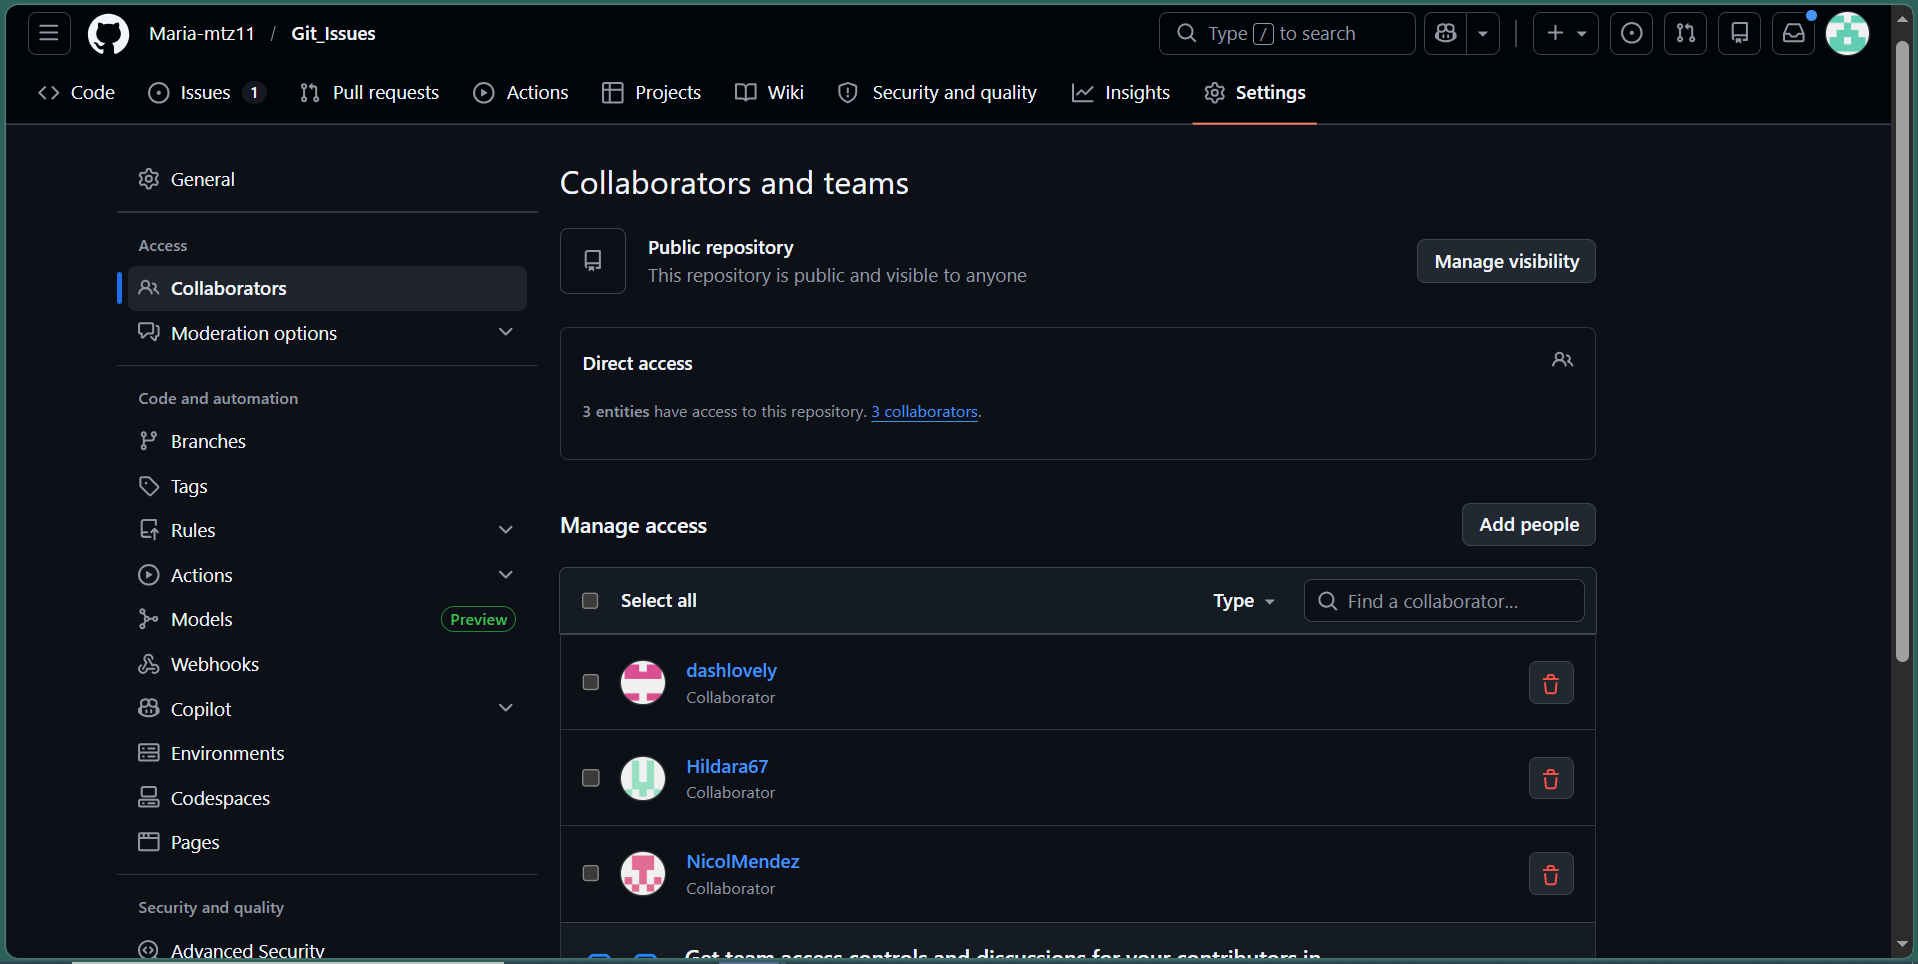
\includegraphics[width=15cm]{imagenes/repositorio.png}
\caption{Repositorio creado en GitHub.}
\label{fig:repositorio}
\end{figure}

\subsection{Creación del Issue}

Se creó un Issue para reportar una problemática detectada dentro del proyecto utilizando GitHub CLI.

\textbf{Título del Issue:}

\begin{quote}
Error en lectura UART
\end{quote}

\textbf{Descripción:}

\begin{quote}
La comunicación serial falla al iniciar el sistema.
\end{quote}

La incidencia fue registrada correctamente en el repositorio, permitiendo documentar el problema y dar inicio al flujo de trabajo colaborativo para su seguimiento y resolución.

\begin{figure}[H]
\centering
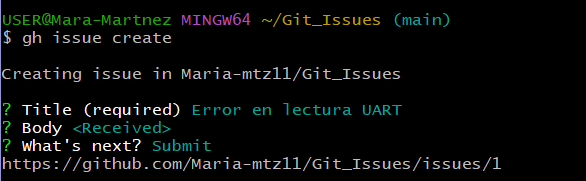
\includegraphics[width=15cm]{imagenes/creación.png}
\caption{Creación del Issue mediante GitHub CLI.}
\label{fig:creacion}
\end{figure}

\subsection{Visualización de Issues}

Para visualizar los Issues registrados se utilizó GitHub CLI mediante el siguiente comando:

\begin{lstlisting}[language=bash]
gh issue list
\end{lstlisting}

Posteriormente se consultó el Issue específico mediante:

\begin{lstlisting}[language=bash]
gh issue view 1
\end{lstlisting}

Esto permitió verificar la información registrada, incluyendo el estado, descripción y responsable de la incidencia.

\begin{figure}[H]
\centering
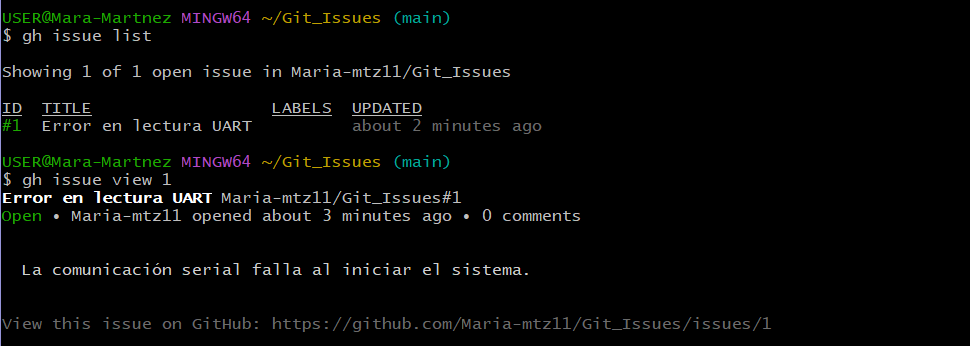
\includegraphics[width=15cm]{imagenes/visualizacion.png}
\caption{Listado y visualización del Issue.}
\label{fig:visualizacion}
\end{figure}

\subsection{Asignación del Issue}

Uno de los integrantes del equipo fue asignado como responsable del Issue para atender la incidencia reportada.

La asignación permitió definir claramente quién sería el encargado de resolver el problema y dar seguimiento a las actividades relacionadas con la incidencia.

\begin{figure}[H]
\centering
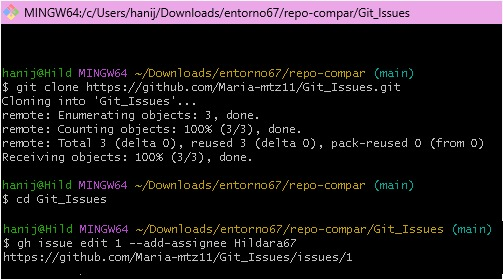
\includegraphics[width=15cm]{imagenes/asignación.jpeg}
\caption{Asignación del Issue a un integrante del equipo.}
\label{fig:asignacion}
\end{figure}

\subsection{Comentarios y seguimiento}

Otro integrante agregó comentarios al Issue para dar seguimiento al avance de la actividad y así mantener comunicación con el resto del equipo.

Ejemplo de comentario realizado:

\begin{quote}
Estoy revisando el problema.
\end{quote}

\begin{figure}[H]
\centering
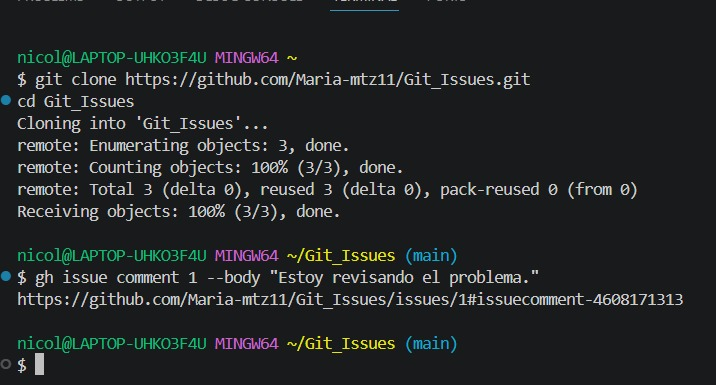
\includegraphics[width=0.9\textwidth]{imagenes/comentario.jpeg}
\caption{Comentario agregado al Issue.}
\label{fig:comentario}
\end{figure}

\subsection{Corrección de la incidencia}

Con el objetivo de simular la resolución de la incidencia reportada, se realizaron modificaciones en el repositorio y posteriormente se registraron los cambios mediante Git.

Para ello se ejecutaron los siguientes comandos:

\begin{lstlisting}[language=bash]
git add README.md
git commit -m "Correccion del issue #1"
git push origin main
\end{lstlisting}

Una vez realizados los cambios, estos fueron almacenados en el historial del repositorio mediante un commit y posteriormente enviados al repositorio remoto para que todos los integrantes del equipo pudieran acceder a la versión actualizada del proyecto.

\begin{figure}[H]
\centering
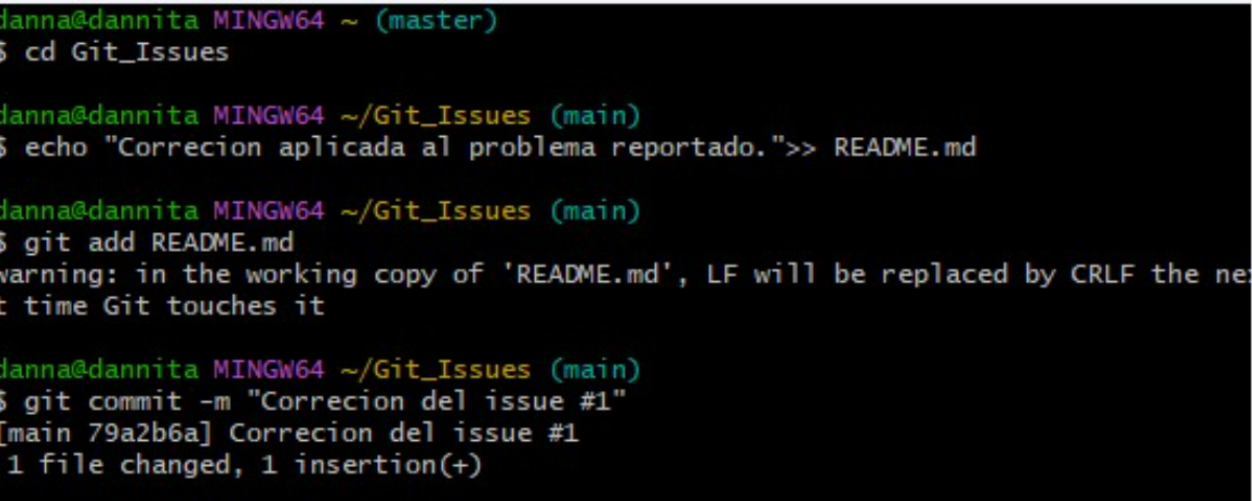
\includegraphics[width=0.9\textwidth]{imagenes/corrección.png}
\caption{Commit realizado para registrar la solución de la incidencia.}
\label{fig:correccion}
\end{figure}

\begin{figure}[H]
\centering
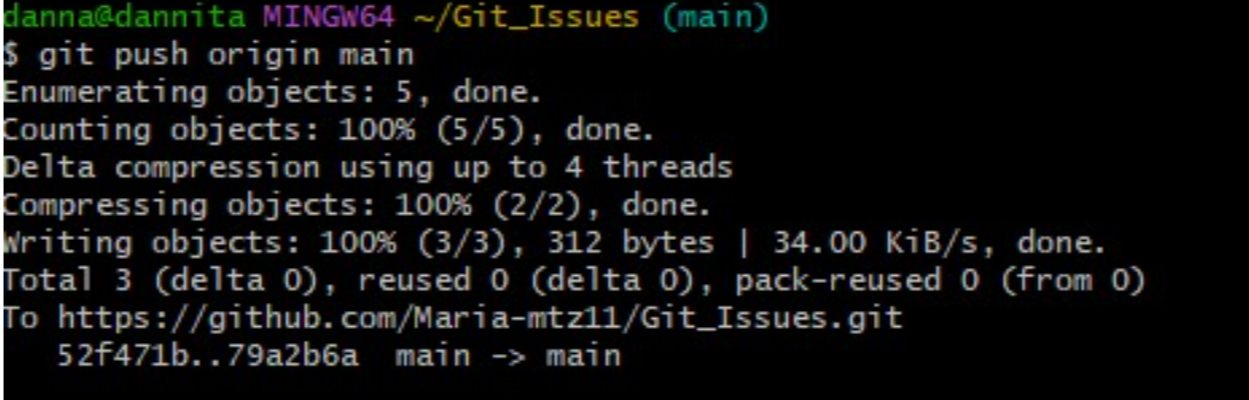
\includegraphics[width=0.9\textwidth]{imagenes/cambios.png}
\caption{Envío de los cambios al repositorio remoto mediante Git Push.}
\label{fig:cambios}
\end{figure}

\subsection{Cierre del Issue}

Una vez solucionado el problema, se procedió al cierre del Issue utilizando GitHub CLI.

\begin{lstlisting}[language=bash]
gh issue close 1
\end{lstlisting}

Con ello la incidencia quedó marcada como resuelta dentro del repositorio.

\begin{figure}[H]
\centering
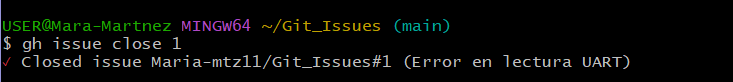
\includegraphics[width=0.9\textwidth]{imagenes/cierre.png}
\caption{Issue cerrado exitosamente.}
\label{fig:cierre}
\end{figure}
\section{Resultados obtenidos}

Durante la práctica se logró implementar correctamente un flujo de trabajo basado en GitHub Issues. Los integrantes del equipo colaboraron en la creación, asignación, seguimiento y resolución de una incidencia reportada dentro del repositorio compartido.

Se registró un Issue relacionado con un error en la lectura UART, el cual fue asignado a un integrante del equipo para su atención. Posteriormente se agregaron comentarios de seguimiento, se realizaron modificaciones en el repositorio y finalmente se cerró la incidencia una vez completadas las actividades correspondientes.

Asimismo, se comprobó el funcionamiento de GitHub CLI como herramienta para la administración de incidencias desde la terminal.
\section{Conclusiones}

GitHub Issues es una herramienta fundamental para la organización de proyectos de desarrollo de software, ya que permite registrar incidencias, asignar responsables y dar seguimiento a las tareas pendientes.

La práctica permitió comprender el flujo de trabajo colaborativo utilizado en entornos reales de desarrollo, así como reforzar el uso de GitHub CLI para la gestión eficiente de incidencias.

Además, se comprobó la utilidad de GitHub Issues para coordinar actividades entre varios integrantes, facilitando la comunicación, el seguimiento de tareas y la documentación de problemas dentro de un proyecto compartido.

\end{document}